\documentclass[journal]{IEEEtran}
\usepackage{graphicx}
\usepackage{listings}
\usepackage[]{units}
\usepackage[style=authoryear,backend=bibtex]{biblatex}
\bibliography{bibtex/bib/crimpbit}
\usepackage{caption}
\usepackage{subcaption}
\usepackage[thmmarks,thref]{ntheorem}
\newtheorem{hyp}{Hypothesis}

\lstset{
    breaklines=true,
}
%\usepackage[english]{babel}
\ifCLASSINFOpdf
  % \usepackage[pdftex]{graphicx}
  % declare the path(s) where your graphic files are
  % \graphicspath{{../pdf/}{../jpeg/}}
  % and their extensions so you won't have to specify these with
  % every instance of \includegraphics
  % \DeclareGraphicsExtensions{.pdf,.jpeg,.png}
\else
  % or other class option (dvipsone, dvipdf, if not using dvips). graphicx
  % will default to the driver specified in the system graphics.cfg if no
  % driver is specified.
  % \usepackage[dvips]{graphicx}
  % declare the path(s) where your graphic files are
  % \graphicspath{{../eps/}}
  % and their extensions so you won't have to specify these with
  % every instance of \includegraphics
  % \DeclareGraphicsExtensions{.eps}
\fi
% correct bad hyphenation here
\hyphenation{op-tical net-works semi-conduc-tor}

\begin{document}
%
% paper title
% can use linebreaks \\ within to get better formatting as desired
\title{Classification of Climbing Grab Movements Measured with Myo Armbands}
\author{Peter~Schulz,
        Dario~Treffenfeld-M\"ader
        and~J\"org~Wilhelms}

% The paper headers
\markboth{Report Wearable Computing, Crimp Bit}%
{Shell \MakeLowercase{\textit{et al.}}: Bare Demo of IEEEtran.cls for Journals}

% make the title area
\maketitle


\begin{abstract}
Understanding climbing movements is vital for improving on performing them efficiently. Supporting this process with technology is a relatively new topic. Yet it is seen as having high potential for assisting trainers and experts in their analysis. In this paper, we present a comparison of a set of established classifiers for classifying grab movements typically seen in climbing based on electromyographic signals measured by Myo armbands.  
\end{abstract}
%\begin{IEEEkeywords}
%IEEEtran, journal, \LaTeX, paper, template.
%\end{IEEEkeywords}
%\IEEEpeerreviewmaketitle

\section{Motivation}

Climbing has become a become a popular sport in recent years \autocite{freizeitklettern}. According to the international federation of sport climbing there are over 25 million active sport climbers \autocite{IFSC:figures}. As other sports, climbing includes improving motor skills, strength, endurance, knowledge, etc \autocite{Kajastila:2014:ACI:2611780.2581139}. Professional training consist of repetition cycles during which an experienced trainer observes a climber and gives feedback by commenting on movements \autocite{Ladha:2013:CSA:2493432.2493492}. Video analysis is used occasionally to assist this process. Though, it is rather cumbersome and remains restricted to observation of the visible. Further, research looking into the climbing movements and trying come up with new concerted training approaches is still a rather young discipline, yet \autocite{denk}.

Approaches have been made using technology to support the training process, for example full body motion analysis using a Microsoft Kinect \autocite{Cha201552,Kajastila:2014:ACI:2611780.2581139}. Wearables have also been used for analysing various aspects of climbing movements \autocite{Ladha:2013:CSA:2493432.2493492} or have been at least suggested \autocite{Kalyanaraman:2015:ARC:2800835.2800856}. So far no efforts have been made to look into the finger grab movements. The fingers are of special interest since they exhaust quickly and are most vulnerable to injuries \autocite{Wright01062001}. Hence analyzing finger movements in sport climbing might help to recognize potentially harmful ones earlier.

\section{Concept}

\subsection{How the Myo Armbands Work}
Electromyography (EMG) is the investigation of the electrical function of the muscles of the human body. If a muscle is contracted there is a measurable muscle response or electrical activity triggered by the nerves of the muscle.

The intramuscular method needs direct access to the nerves (by a needle or other instruments). This method is used by neuromedicine to detect neuromuscular deviation \autocite{neuromedicine}. Deviations of the electrical activity can for example indicate diseases of the muscle or nerves. This method is not recommandable for this project, because there is always a risk of infections or other harms to the proband.

On the surface of the muscles you can also measure electrical activity. This method, called surface EMG, is less accurate because it is harder to precisely recognize the muscle that was moved, or the nerve that was used to trigger the muscle activity \autocite{myoUniGoettingen}. The Myo gesture control armband works with surface EMG, but the data delivers appropriate readings for this project.

\subsection{Hypothesis}

\begin{hyp}\label{hyp:subject}
$H_{0_{\thehyp}}$: The classification accuracy is independent of the test subject hence it does not make a difference if only one classifier is used for all test subjects or if one classifier is used per test subject.

A classifier trained per test subject yields significantly more accurate results than a classifier trained on all test subjects.
\end{hyp}

\begin{hyp}\label{hyp:direction}
$H_{0_{\thehyp}}$: The classification accuracy is independent of the pull direction hence it does not make a difference if only one classifier is used for all pull directions or if one classifier is used per pull direction.

A classifier trained per pull direction yields significantly more accurate results than a classifier trained on all pull directions.
\end{hyp}

\begin{hyp}\label{hyp:arm}
$H_{0_{\thehyp}}$: The classification accuracy is independent of the arm hence it does not make a difference if only one classifier is used for both arms or if one classifier is used per arm.

A classifier trained arm yields significantly more accurate results than a classifier trained on both arms.
\end{hyp}

\subsection{Getting Data to Test On}

\subsubsection{Record Data}

To record data for the evaluation a software must was written for that purpose. This program provides a graphical user interface which allows to manage subjects an there attributes next to recordings. It can visualize the data for visual inspection. It allows for recordings of discrete length.

\subsubsection{Preprocessing Data}

The conducted tests are based on recordings of EMG signals measured and broadcast by a Myo armband at \unit[200]{Hz} \autocite{myo-emg}. Since Bluetooth LE cannot cope with this frequency, a Myo sends 2 sets of 8 bytes at the maximum rate. Each sample is rather small and could be seen as a 2x8 pixel gray-scale image. As for this we decided to omit a dedicated feature selection and instead consider each sensor value as a relevant feature for the time being.

However, each sensor value gets preprocessed as follows. 1) all signals are run through an envelope follower filter to get rid of the oscillation and to smooth peaks. 2) The signal stream is split into chunks of $n_c$ samples which are compressed to the mean value of this chunk. 3) Each mean value is mapped to an interval indexed from $0$ to $n_i$. The larger $n_c$ the more samples are considered for one mean value and less instances can be extracted from one recording. When $n_i$ grows the number of possible values for an instance attribute decreases. Choosing appropriate values for $n_c$ and $n_i$ is part of the evaluation process.

\subsubsection{Data Analysis with Weka\footcite{weka}}
After preprocessing the data it will be given to different weka algorithms to find the best one for climbing gesture recognition. This classifiers are trained on different data sets. 

For every test run the chosen data to train the classifiers is different. With the different data sets the best classifier for different subjects, arms and pull directions can be determined.

\section{Experimental Setup}
The experiment was executed with 1 person at a time to make sure gestures, tags and arms are assigned correctly. The experiment was executed with 5 probands aged between 18 and 34, 1 proband female, 4 male.

The experiment was split into different test locations. 4 tests were executed as a field test in a climbing hall and 1 test was executed as laboratory test.

At the beginning the proband had to take on 2 Myo gesture control armbands, so the armbands could warm up and the tester could ensure that the assignment of the arm to the armbands was correct. A simple ping in the analysis application was used to determine the correct arm.

The proband had to do all gestures from figure \ref{gestures} for every pull direction from figure \ref{tags}. The gestures determine the amount of fingers used (and which fingers are used) and the pull direction determines the direction, in which the proband has to pull.

Before each gesture was started, the tester told the proband what he had to do, let the proband start the current gesture in the current pull direction, started the recording and after the recording was done, told the proband to release the gesture.

\begin{figure*}[t!]
    \centering
    \begin{subfigure}{0.25\textwidth}
        \centering
        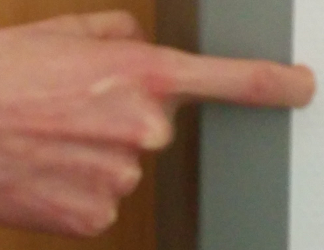
\includegraphics[width=.8\linewidth]{img/index}
        \caption{index}
    \end{subfigure}%
        \begin{subfigure}{0.25\textwidth}
        \centering
        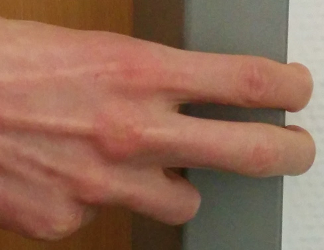
\includegraphics[width=.8\linewidth]{img/index+middle}
        \caption{index+middle}
    \end{subfigure}%
        \begin{subfigure}{0.25\textwidth}
        \centering
        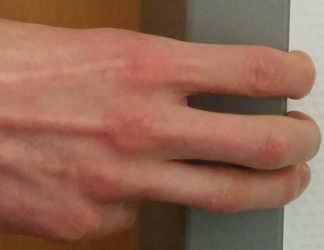
\includegraphics[width=.8\linewidth]{img/index+middle+ring}
        \caption{index+middle+ring}
    \end{subfigure}%
    
    
        \begin{subfigure}{0.25\textwidth}
        \centering
        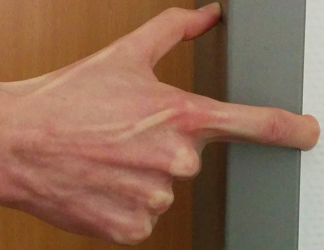
\includegraphics[width=.8\linewidth]{img/index+thumb}
        \caption{index+thumb}
    \end{subfigure}%
    \begin{subfigure}{0.25\textwidth}
        \centering
        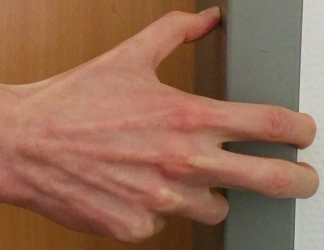
\includegraphics[width=.8\linewidth]{img/index+middle+thumb}
        \caption{index+middle+thumb}
    \end{subfigure}%
        \begin{subfigure}{0.25\textwidth}
        \centering
        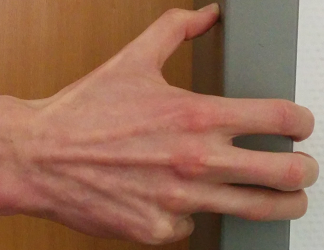
\includegraphics[width=.8\linewidth]{img/index+middle+ring+thumb}
        \caption{index+middle+ring+thumb}
    \end{subfigure}%
    \caption{Gestures} \label{gestures}
\end{figure*}

\begin{figure*}[t!]
    \begin{subfigure}{0.25\textwidth}
        \centering
        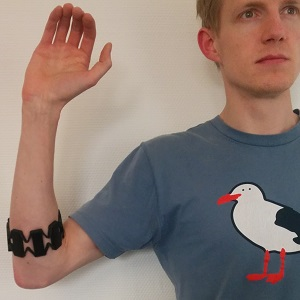
\includegraphics[width=.8\linewidth]{img/pull-downwards}
        \caption{pull-downwards}
    \end{subfigure}%
        \begin{subfigure}{0.25\textwidth}
        \centering
        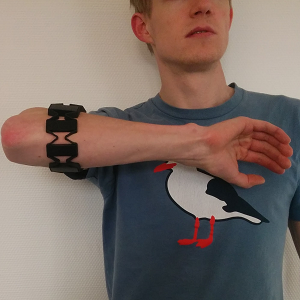
\includegraphics[width=.8\linewidth]{img/pull-gaston}
        \caption{pull-gaston}
    \end{subfigure}%
        \begin{subfigure}{0.25\textwidth}
        \centering
        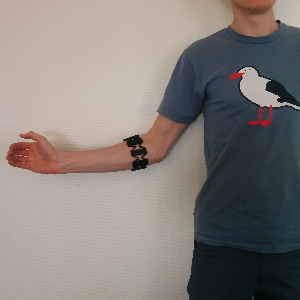
\includegraphics[width=.8\linewidth]{img/pull-sideways}
        \caption{pull-sideways}
    \end{subfigure}%
        \begin{subfigure}{0.25\textwidth}
        \centering
        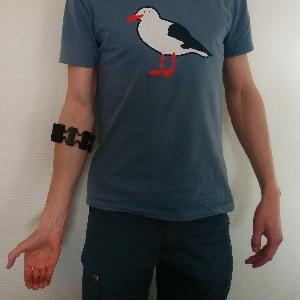
\includegraphics[width=.8\linewidth]{img/pull-upwards}
        \caption{pull-upwards}
    \end{subfigure}%
    \caption{Pull Directions} \label{tags}
\end{figure*}
    
\section{Implementation}
\subsection{Receiving Data}
The Myo SDK \autocite{myosdk} provides access to several gestures that are recognized. These gestures are not applicable to recognition of climbing processes. The Myo armband also provides raw EMG data from 8 different EMG Sensors with redundant data that allows to evaluate the data by oneself. Each sensor provides a byte value that needs to be processed.
\subsection{Experience}
\begin{itemize}
 \item automatic detection of arm unreliable
 \item difficult to get reproducible process for all probands
\end{itemize}

\section{Evaluation}

\subsection{Classifiers}
A classifier is an algorithm that predicts the type, label, name or class of a given datum. In this project we use algorithms using Naive Bayes, Logistic Regression, Decision Trees and Support Vector Machine to classify the data.\autocite{machine_learning}
\subsubsection{NaiveBayes}
The NaiveBayes classifier assigns a data set either the class with the highest probability to be the right on, or the one it\rq{}s cheapest to assign it to. Computing the likelihood that a dataset is from a given class can be done in linear time and is faster than Logistic Regression, Decision Trees or Support Vector Machine. \autocite{ibm}
\subsubsection{J48 (C4.5 algorithm)}
J48 is a Java implementation of the C4.5 algorithm. The J48 takes the training data and generates a decision tree from it. The classifier can now classify the test set instance by going down the branches of the decision tree that match the test instance. \autocite{top10}
\subsubsection{Logistic}
The Logistic classifier is the Weka implementation that uses Logistic Regression. Logistic Regression builds a function that calculates the probability for an specific outcome. \autocite{top10}
\subsubsection{Support Vector Machine}
We use LibSVM as our Support Vector Machine classifier. The classes in the training set are divided by an hyperplane $f(x)$. Once the data is divided the test data set $x_n$ is passed to the function, we kann now see the predicted class form the result.
\autocite{top10}

\subsection{Data structure}

The myo armband sends the values for all of it\rq{}s 8 emg sensors multiple times a second. For our test we also know the test subject, the pull direction (pull-downwards, pull-upwards, pull-sideways, pull-gaston), the arm (left or right) and the combination of fingers that were used (index, index+middle, index+middle+ring, index+thumb, index+middle+thumb ,index+middle+ring+thumb).
We have to translate this data into a data structure supported by Weka.
Weka works with \texttt{Instances}, \texttt{Instance} and \texttt{Attribute}. An \texttt{Attribute} is in our case either an emg value or a combination of fingers. We combine emg values and the combination of fingers that happed at the same point in time together into an \texttt{Instance}. This \texttt{Instance} looks something like this:
\begin{verbatim}
4,3,3,3,3,3,3,4,index
\end{verbatim}
The \texttt{Instances} contains all of our \texttt{Instance} Objects. Weka saves this \texttt{Instances} in an *.arff file, which is human readable:

\begin{lstlisting}
@attribute emg_0 numeric
...
@attribute emg_7 numeric
@attribute grip_type {index, ...}

@data
3,3,3,3,3,3,3,3,index
...
4,3,3,3,3,3,3,4,index+middle+ring+thumb
\end{lstlisting}

This data structure can now be used by Weka.

\subsubsection{Training set and Test set}

Each classifier is trained on a training set and tested against a test set. Both sets are created from the same set of recordings. In order to get two distinct sets of instances each recording is split. The training set is generated of the first 80\% of every recording meanwhile the test set comes from the remaining 20\%. Other ways Of splitting a recording, for example picking the test portion randomly, have been considered but not tested for the sake of simplicity.
The training data gets normalized by subtracting the mean of all values from each value and dividing the difference by the standard deviation of all values. Both mean and standard deviation of the training set are used to normalize the training data, too. 

\subsubsection{Classifier Assessment}

In order to compare classifiers they are each assessed separately based on the same data. First, cross Validation is used to measure the accuracy on the training set. Each training set is randomly cross validated using 10 folds. This way an average of 16, at least 8, randomly picked instances is tested against the remaining instances. The test results of all 10 folds are summarized as one classifier evaluation. Second, for a real life scenario each trained classifier is run against the unseen instances of the test set which results in another classifier evaluation.

\subsubsection{Filtering the Data}

Our raw data is filterd by 3 filter before given to the classifier. The first filter is an envelop filter. This filter smooths the data and converts every negative value into a positive one. 
The second filter is an average filter. It condenses $n_c$ EMG values into one average value.
The third filter is a label filter. We give the filter the variable $n_i$ and it converts each EMG value to one of $n_i$ labels.    

\subsection{Running the Tests}

The tests where run in two phases. During the first phase the aforementioned filter parameters $n_c$ and $n_i$ where determined. These parameters where then used in the second phase where multiple classifiers where trained on different training sets and compared with each other.

\subsubsection{Filter Parameters}

To figure out good chunk size $n_c$ and number of intervals $n_i$ one and the same test was run several times testing different combinations of $n_c$ and $n_i$. The test was a cross validation of the complete training set including all recordings. We choose $n_i$ to run from 0 (no filtering) to 20 and $n_c$ from 0 (no filtering) to 30. The results vary depending on the classifier, see Table \ref{tab:filterparameters}. 

\begin{table}
\centering
\begin{tabular}{lccc}
\textbf{Classifier} & \textbf{$n_c$} & \textbf{$n_i$} & \textbf{Accuracy (in \%)} \\
\hline
LibSVM & 15 & 26 & 82.65\\
J48 & 14 & 16 & 80.61\\
Logistic & 15 & 16 & 73.46\\
NaiveBayes & 16 & 16 &  61.22\\
\end{tabular}
\caption{Preprocessing filter parameters $n_c$ (chunk size) and $n_i$ (number of intervals)}
\label{tab:filterparameters}
\end{table}

\subsubsection{Hypothesis Testing}

In order to test \thref{hyp:subject} a classifier was trained for each combination of arm and pull direction with recordings from all subjects. Another batch of classifiers was trained for each combination of arm, pull direction, and subject. All evaluation results where analyzed using a Two-Way ANOVA. The number of subjects per training set and the classifier where chosen as factors. This method might be error prone as stated by \citeauthor{ref1} since it ignores that the conducted tests are not independent. Still, the results should suffice as an indicator. Table \ref{tab:anova} shows the results of the comparison. Both, cross validation accuracy and test accuracy off all classifiers examined are significantly higher when the classifier is trained per subject, see also Table \ref{tab:anova-mean-cv-difference} and \ref{tab:anova-mean-test-difference} and Figure \ref{fig:anova-mean-test}. Regarding the factor "number of subjects per training set", J48 produced the highest p-value with 0.024 followed by LibSVM with 0.011. Whereby a higher p-value indicates a smaller variance between the groups of each factor. This disproves $H_{0_{\ref{hyp:subject}}}$ and thereby supports \thref{hyp:subject}.

\thref{hyp:direction} was tested in a similar fashion. Notably the difference of means for both cross validation accuracy and test accuracy is almost half a low as for as for the previous test. Which means that there are smaller differences in-between classifiers. Since all examined classifiers produced significantly better results when trained with a more specialized training set \thref{hyp:direction} becomes unlikely, too.

Finally \thref{hyp:arm} was tested the same way as the other hypothesis before. At first glance a comparison based on the factor "number of arms per training set" the still shows significant differences between the two possible characteristics. However, looking at the comparison based on the same factor within each classifier, there is almost no significant difference. As can be seen in Table \ref{tab:anova-arm}, only NaiveBayes produces a significantly different cross validation accuracy depending on the number of arms it was trained on. For the test accuracy none of the classifiers produced any significant difference. Hence $H_{0_{\ref{hyp:arm}}}$ might be likely after all.

\begin{table}
\centering
\begin{tabular}{llrrr}
\textbf{Test $X$} & \textbf{Method} & \textbf{$\Delta$ Means} & \multicolumn{1}{l}{\textbf{t}} & \multicolumn{1}{l}{\textbf{P}} \\
\hline
subject                                    & CV              & 19.808                 & 11.485                         & \textless0.001                 \\
subject                                    & Test            & 18.657                 & 8.181                          & \textless0.001                 \\
pull direction                             & CV              & 12.769                 & 7.430                          & \textless0.001                 \\
pull direction                             & Test            & 10.849                 & 4.798                          & \textless0.001                 \\
arm                                        & CV              & 5.884                  & 4.460                          & \textless0.001                 \\
arm                                        & Test            & 4.720                  & 2.814                          & 0.005
\end{tabular}
\caption{Two-Way ANOVA comparison of cross validation (CV) and test accuracy (in \%) based on the factor "number of $X$ in training set". Each row compares one classifiers trained on all $X$ vs on trained per $X$.}
\label{tab:anova}
\end{table}

\begin{table}
\centering
\begin{tabular}{lrrr}
\textbf{Classifier} & \textbf{$\Delta$ Means} & \multicolumn{1}{l}{\textbf{t}} & \multicolumn{1}{l}{\textbf{P}} \\
\hline
LibSVM              & 1.752                  & 0.664                          & 0.507                          \\
J48                 & 3.850                  & 1.459                          & 0.146                          \\
Logistic            & 4.307                  & 1.632                          & 0.104                          \\
NaiveBayes          & 13.626                 & 5.164                          & \textless0.001                
\end{tabular}
\caption{Two-Way ANOVA comparison cross validation accuracy (in \%) based on number of arms in training set within the examined classifiers}
\label{tab:anova-arm}
\end{table}

\begin{table*}[t]
\centering
\begin{tabular}{lrrrrrr}
\textbf{Classifier} & \textbf{Subject CV} & \multicolumn{1}{l}{\textbf{Subject Test}} & \multicolumn{1}{l}{\textbf{Direction CV}} & \multicolumn{1}{l}{\textbf{Direction Test}} & \multicolumn{1}{l}{\textbf{Arm CV}} & \multicolumn{1}{l}{\textbf{Arm Test}} \\
\hline
LibSVM              & 82.210            & 76.468                                  & 82.405                                  & 78.246                                    & 85.999                            & 80.790                              \\
J48                 & 74.513            & 70.016                                  & 74.995                                  & 70.944                                    & 76.816                            & 74.067                              \\
Logistic            & 67.678            & 64.357                                  & 72.171                                  & 68.941                                    & 76.406                            & 72.367                              \\
NaiveBayes          & 66.751            & 63.436                                  & 74.816                                  & 71.763                                    & 79.059                            & 74.927                              \\
\hline
Std Err of LS Mean  & 1.725               & 2.281                                     & 1.719                                     & 2.261                                       & 1.319                               & 1.678                                
\end{tabular}
\caption{Two-Way ANOVA comparison grouped mean accuracy (in \%) of the examined classifiers for different factors. These mean values contain results from $H_0$ training sets and their counterparts.}
\label{tab:anova-mean-accuracy}
\end{table*}


\begin{table*}
\centering
\begin{tabular}{lrrrrrrrrrrr}
                      & \multicolumn{3}{c}{Subject}                                                      & \multicolumn{3}{c}{Direction}                                                    & \multicolumn{3}{c}{Arm}                                                           & \multicolumn{1}{l}{}            & \multicolumn{1}{l}{}                       \\
\textbf{}             & \multicolumn{1}{l}{All} & \multicolumn{1}{l}{One} & \multicolumn{1}{l}{$\Delta$} & \multicolumn{1}{l}{All} & \multicolumn{1}{l}{One} & \multicolumn{1}{l}{$\Delta$} & \multicolumn{1}{l}{Both} & \multicolumn{1}{l}{One} & \multicolumn{1}{l}{$\Delta$} & \multicolumn{1}{l}{\O $\Delta$} & \multicolumn{1}{l}{\O $\Delta$ $\sigma^2$} \\ \hline
\textbf{J48}        & 69,74                                     & 79,29                                    & 9,56                               & 71,01                                       & 78,98                                      & 7,97                               & 74,89                                  & 78,74                                & 3,85                               & 7,12                                    & 2,95                                           \\
\textbf{NaiveBayes} & 47,68                                     & 85,82                                    & 38,14                              & 63,53                                       & 86,10                                      & 22,57                              & 72,25                                  & 85,87                                & 13,63                              & 24,78                                   & 12,41                                          \\
\textbf{LibSVM}     & 77,64                                     & 86,78                                    & 9,14                               & 78,01                                       & 86,80                                      & 8,78                               & 85,12                                  & 86,88                                & 1,75                               & 6,56                                    & 4,16                                           \\
\textbf{Logistic}   & 56,48                                     & 78,88                                    & 22,40                              & 66,29                                       & 78,05                                      & 11,76                              & 74,25                                  & 78,56                                & 4,31                               & 12,82                                   & 9,09                                           \\ \hline
SEM        & 3,12                                      & 1,47                                     &                                    & 3,07                                        & 1,54                                       &                                    & 2,12                                   & 1,58                                 &                                    &                                         &                                               
\end{tabular}
\caption{Two-Way ANOVA comparison of mean cross validation accuracy (in \%) between the two levels of factor "number of X in test set"}
\label{tab:anova-mean-cv-difference}
\end{table*}

\begin{table*}
\centering
\begin{tabular}{lrrrrrrrrrrr}
                      & \multicolumn{3}{c}{Subject}                                                      & \multicolumn{3}{c}{Direction}                                                    & \multicolumn{3}{c}{Arm}                                                           & \multicolumn{1}{l}{}            & \multicolumn{1}{l}{}                       \\
\textbf{}             & \multicolumn{1}{l}{All} & \multicolumn{1}{l}{One} & \multicolumn{1}{l}{$\Delta$} & \multicolumn{1}{l}{All} & \multicolumn{1}{l}{One} & \multicolumn{1}{l}{$\Delta$} & \multicolumn{1}{l}{Both} & \multicolumn{1}{l}{One} & \multicolumn{1}{l}{$\Delta$} & \multicolumn{1}{l}{\O $\Delta$} & \multicolumn{1}{l}{\O $\Delta$ $\sigma^2$} \\ \hline
\textbf{J48}        & 64,80 & 75,23 & 10,43 & 66,66 & 75,30 & 8,64  & 72,90 & 75,23 & 2,33  & 7,13  & 4,26  \\
\textbf{NaiveBayes} & 46,49 & 80,38 & 33,89 & 63,14 & 80,38 & 17,24 & 69,47 & 80,38 & 10,91 & 20,68 & 11,87 \\
\textbf{LibSVM}     & 70,58 & 82,36 & 11,78 & 74,14 & 82,36 & 8,22  & 79,22 & 82,36 & 3,13  & 7,71  & 4,34  \\
\textbf{Logistic}   & 55,09 & 73,62 & 18,53 & 64,26 & 73,62 & 9,37  & 71,11 & 73,62 & 2,51  & 10,14 & 8,04  \\ \hline
SEM        & 4,13  & 1,95  &       & 4,05  & 2,02  &       & 2,69  & 2,01  &       &       &
\end{tabular}
\caption{Two-Way ANOVA comparison of mean test accuracy (in \%) between the two levels of factor "number of X in test set"}
\label{tab:anova-mean-test-difference}
\end{table*}

\begin{figure}
\centering
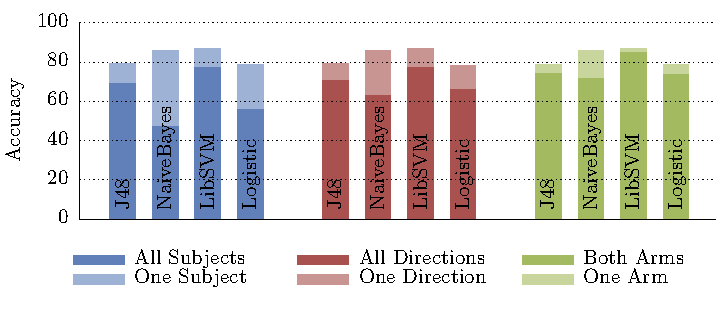
\includegraphics[width=\linewidth]{img/avg-accuracy-test-wrapped.pdf}
\caption{Two-Way ANOVA comparison of mean test accuracy (in \%) for all examined classifiers}
\label{fig:anova-mean-test}
\end{figure}

\section{Conclusion and Future Work}

We have presented a comparison of a set established classifiers for classifying typical grab gestures used in climbing based on EMG signals measured at the underarm. The results imply the chance of classifying a gesture correctly in this scenario are dependent on test subject and pull direction but is invariant with regard to the arm the sensor is worn. Simply put, a set of classifiers trained subject might improve the classification accuracy. If this set contains classifiers which are picked depending on the pull direction, which could be determined based on the IMU signals of the Myo, this might increase the classification accuracy even further. On the other hand, having a classifier for each arm is unlikely to improve the classification accuracy. Looking at Table \ref{tab:anova-mean-accuracy} an SVM based classifier appears to produce the most accurate results.

Our findings are just a small step towards a better understanding of movements in climbing and their analysis. We encourage other to delve into this topic, for example, by examining potentially harmful grab movements and try to recognize them. Considering the body weight of subjects would be another option. It could be examined if the weight of a subjects or the portion of that weight lifted while grabbing and pulling has any influence on the classification results. We further propose combining the Myo based grab movement analysis with other sensors for full body motion tracking for obtaining a better understanding of climbing movements, for example, how they influence the position of the center of gravity which plays an important role.

\section{Acknowledgments}

This work was made possible by the working group of Prof. Lawo which provided us with the Myo armbands. This goes as well for the DAV Kletterzentrum Bremen for allowing us to use their climbing gym.

\appendices

\printbibliography

\end{document}